% Chapter 1

\chapter{Prototype I} % Main chapter title

\label{prototype1chapter} % For referencing the chapter elsewhere, use \ref{Chapter1} 

\lhead{Chapter \emph{Prototype I}} % This is for the header on each page - perhaps a shortened title
%----------------------------------------------------------------------------------------
\section{Development of the Prototype}
The initial task was to develop the first version of the application prototype. The prototype had features that allow monitoring of physical activity and diet of an individual. The manipulation of user interfaces of the app was specifically targeted to help givers/intermediary users. The prototype was designed to encourage one help-giver to work together with one help-seeker by forming one pair of users. In order to make the act of helping to be perceived as both important and meaningful by intermediary users, the first message displayed when opening the app was explicit that an intermediary user is helping someone they know to manage their wellness. In the case of motivating ongoing use, the app had included gamification features of where each pair could be awarded points, badges, nice looking gardens, and fish tanks. The essence of having these features was to enable pairs of users to have a set of challenges that will promote competence which is one of the core aspects of self-determination theory. In addition to the aforementioned features, within each pair of users' garden and fish tank, there was a Facebook social plug-in that could allow members from different teams/pairs to comment on or like each other. The presence of these social features was to promote relatedness which is also one of the aspects of self-determination theory. Facebook groups were also utilized to give feedback or remind users to engage with the application. The first prototype didn't explicitly have any functionality to support autonomy. Ideally, the information flow on the high-level representation of the system to encourage intermediated use was designed as depicted on Figure \ref{figure:prototype_1}. A web app was developed using a combination of several web technologies such as HTML, JQuery, JavaScript, and CSS on the client side while the server side was implemented using Django Python framework. Sample screen-shots of the prototype are shown on Figure \ref{figure:prototype_1_screens}. Authentication was done through Facebook accounts of intermediary users. 

\begin{figure}[htbp]
  \centering
    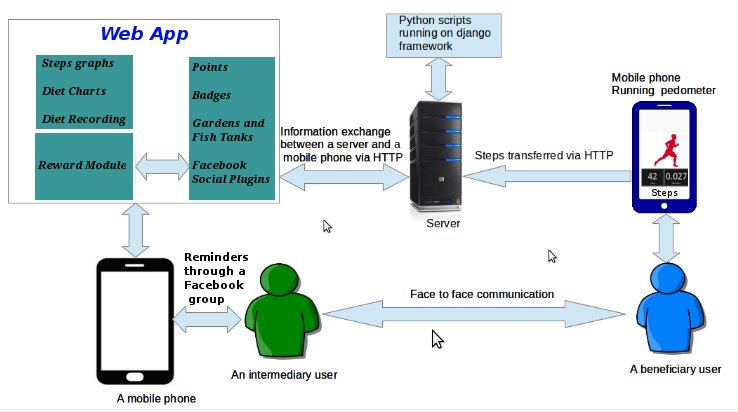
\includegraphics[width=0.8\textwidth]{Figures/prototype_1.png}
    \rule{35em}{0.5pt}
  \caption{Information flow in the first prototype.}
  \label{figure:prototype_1}
\end{figure}

\begin{figure}[htbp]
  \centering
    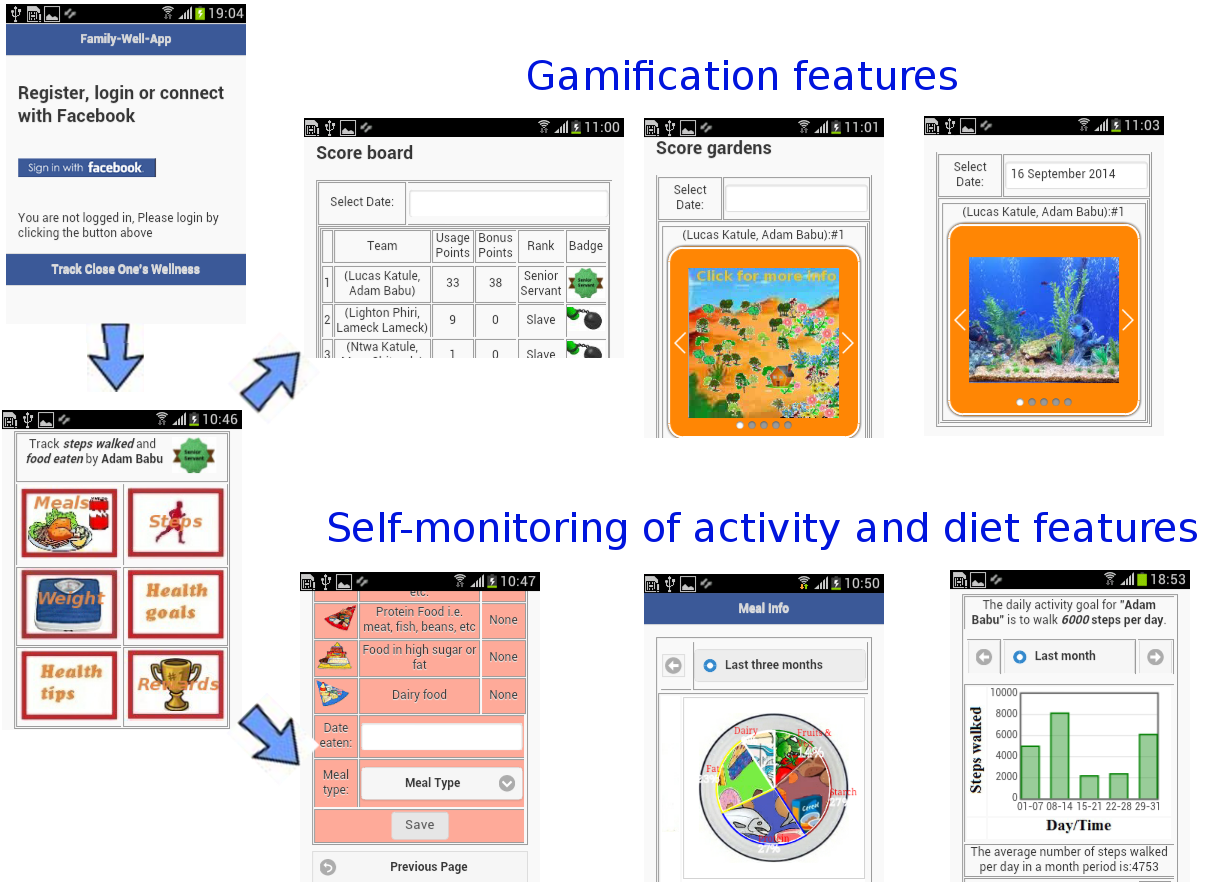
\includegraphics[width=0.8\textwidth]{Figures/Version1/Prototype1Screenshots.png}
    \rule{35em}{0.5pt}
  \caption{Sample screen-shots of the first prototype}
  \label{figure:prototype_1_screens}
\end{figure}

This prototype aimed at encouraging increase in physical activity and  decrease of sedentary behaviours through informing individuals (help-seekers) of their current behaviour trends. In addition, also individuals could monitor whether they were eating healthy or not. Some visualization techniques that are similar to this have been previously used  in systems that were designed for direct users such as ``Fish'n'Steps''\citep{lin2006:fish}, ``Ubifit''\citep{klasnja2009:using},  and ``Few Touch Application''\citep{arsand:mobile}. The idea of using a plate to showing distribution of meals' nutrition mimicked a practice that was used by dietitians at the hospital were we conducted the contextual inquiry reported in the previous chapter. In this design metaphor, the amount of each food group that needs to be consumed is presented as a bisector of a pie chart. 
\section{Prototype Evaluation}
There was a slightly change of plan  due to contention about the study design and implications to ethics when dealing with patients as per requirements of Faculty of Health Sciences Human Research Ethics Committee (FHS-HREC) of University of Cape Town. FHS-HREC was interested to have clinical outcomes as one of the expected outputs. These requirements were going to increase the scope of the work of which its main area of contribution was supposed to be in human-computer interaction. Also, the envisaged technology was only under research; hence it was not expected to be comprehensive enough and ready for any clinical trials even after completions of all evaluations that were meant to be carried out throughout this research. Therefore, I had to look for a different group of participants outside hospital settings. This involved reapplication of ethical approval to an institution body different from the first one that approved the study reported in the previous chapter. The ethical approval was obtained from Faculty of Science Research Ethics Committee (FSREC) of University of Cape Town (see Appendix \ref{AppendixB}).

In order to evaluate the aforementioned prototype, I recruited participants through help from an NGO
based in Cape Town called ``\textbf{\textit{Mamelani Projects}}''\footnote{http://www.mamelani.org.za/}. This NGO was carrying out outreach programs on health education in less privileged
communities. Mamelani was training women on issues of HIV/AIDS, nutrition, and gender equality. 

The NGO helped to recruit participants among people who were part of their trainings in Philippi township. Criteria for recruitment were as follows: (1) participants that were mid-aged and above (contextual enquiry suggested that most prospective beneficiaries could be above mid-aged) and (2) participants must had an intermediary person willing to work with them (someone they trusted or close to them). The NGO identified the targeted participants that met the inclusion criteria. A total of six adult participants were recruited of which both were women above mid-aged (\textgreater= 35 years of age). Each one of the adults brought one intermediary to form a pair. Three intermediaries were girls in between 19-23 years of age. The remaining three intermediaries were boys aged between 14 and 19 years of age. 

Participants were informed of their rights. Participants were also informed of which of their information will be collected by the study. Both adults and their respective intermediaries signed consent forms except for intermediaries who were minors, these signed assent forms that were approved by their respective parents/guardians. 

The next step entailed training of intermediaries on how to use the app. The application was deployed to the field from the end of October 2014 to beginning of December 2014. In order to limit potential complications from deploying the intervention on multiple platforms, each pair of participants was given one Android phone (Samsung GT-S5300) running the pedometer app. Participants were required to utilize the web application hosted at University of Cape Town by using a web browser built into their phones. In order to retain participants in the study each intermediary participant and each beneficiary participant who remained as part of the study received ZAR30 (\~US\$3) worth of airtime every week for the duration of the study. I collected qualitative feedback in the middle and at the end of the study. All the names used in qualitative feedback are just pseudonyms to protect identity of participants.
\section{Findings}
Observations and qualitative feedbacks from the six cases/pairs are presented below. The first three pairs consisted of parents working their children while the remaining three pairs it was just an adult working with either a close or distant relative in each pair.
\subsection*{\textbf{Pair 1: Mother and Son}}
This pair consisted of a boy aged 17 years of age working with his mother. The boy is referred here with the name ``\textbf{Jabulani}'' and his mother is referred with the name ``\textbf{Nandipha}''. Jabulani lived with his mother and other siblings. He appeared to be passionate in engaging with a cellphone. He described the intimate relationship he had with his cellphone.

\userquote{\textbf{Jabulani}} {``There is a time I lost my cellphone. It was like the end of the world to me because I didn't have anything to play with''}

The excerpt above shows that a cellphone could be a source of intrinsic motivation for young users in this context. 

He mentioned that he felt happy helping his mother. He also articulated the reason for helping his mother as that he felt it was his duty since the mother took care of him when he was growing up. 

\userquote{\textbf{Jabulani}} {``I feel happy when I am helping her because she helping me when I was growing up so it is my turn to help her''}

\textbf{Nandipha} also felt very happy being helped by her son and she mentioned that she thinks her son is very brilliant more than her in technology and she gets to know things because of him. 

Jabulani and Nandipha were the first one to engage with the app for at least three different days. All of a sudden their use stopped. When I asked Jabulani together with his mother of challenges that might have prevented them from using the app, their responses indicated that were more conscious about airtime as it was one of the reasons of why they didn't login more often. So there were times where they ran out of airtime. They thought having more data bundles might solve the problem. Another reason for why they didn't use the app more often is associated with lack of competitions from other pairs and also they had accomplished the highest challenge within few days. In the first few days they were so curious about attaining the highest badge. Jabulani claimed that her mother was walking up and down so that they reach that goal. Jabulani discussed with his mother that they must reach that goal in  a week. They managed to reach the goal and there was no more boundary to break.

Badges were one source of motivation to this pair. Jabulani felt motivated by the badges and he was persuading his mother to work harder so that they reach the highest badge which was Queen/King.

\userquote{\textbf{Jabulani}} {``We talked me and my mum that we must not reach only for today but for the whole week. That was our goal to reach the queen and the king for the whole week. I remember a day that was the best day. My mum woke up very early to walk around, to go to Philippi Makasikava [A location within the neighbourhood] just to reach that goal''}

Also Jabulani noticed something on the scoreboard. He and his mother were there leading. Another team (Pair 3) was in the second position. The third position was held by Pair 4. Then after few days Jabulani noticed that Pair 4 moved from a third position to a second position. So Jabulani told his mother that ``we must not drop down because they (Pair 4) are going to reach us''. In that context competition with others was a source of motivation for Jabulani. Although Jabulani was helping his mother but he thought like the ownership of the winning process as theirs because he used the word “We” all the time to imply that he felt that he was part of that process. Additionally, Jabulani enjoyed information displayed by a botanical garden and a fish bowl. He explained why he was so interested in such abstract visualizations. When he was growing up he used to watch cartoons. So when he sees those pictures of trees and fish he feels he is part of that process of making those images/cartoons. So drawing fish and trees through their team's performance motivates him more and he tells his mother that they must have more fish in the bowl. Also the idea of fish in the bowl motivated Nandipha to walk more. She mentioned  that she didn't like to see her bowl empty without any fish, so she tried to walk more steps as she could. These ideas of abstract visualization such as fish bowls/tanks and garden have been previously used in systems that involved only one user on interaction with user interfaces \citep{lin2006:fish, klasnja2009:using}, the only difference in this context is that, the same ideas were extended and tested with two users who were collaborating to attain one objective. 
\subsection*{\textbf{Pair 2: Mother and Son}}
``\textbf{Dumisani}'' was a 14 years of age who lived with his mother, ``\textbf{Kholiwe}''. Dumisani was acting as an intermediary for Kholiwe. Dumisani and Kholiwe used the system for only the first three days and they dropped out. On responding to the question of why was it the case, Kholiwe mentioned that it was the inability to access the system every time they tried out. The web page was always giving them time-outs and this discourages them from trying. But it was also observed that Dumisani was not very familiar with Facebook authentication as he didn't have an account before. I created one account for him of which it wasn't very helpful. The decision in using Facebook authentication was based on an assumption that all intermediaries may have Facebook accounts which was not the case. However, despite technical challenges this pair also showed enthusiasm in using the app.
\subsection*{\textbf{Pair 3: Mother and Daughter}}
``\textbf{Zama}'' who was a 20 years of age was supposed to act as an intermediary for her mother, ``\textbf{Fikile}''. Since the daughter appeared to be interested to help her mother, then one would think that intermediation is possible. Unfortunately, the two lived in different houses and they never used the system at all. Their contact to discuss issues about the system was limited as Zama was raising a toddler at that time. In addition, Fikile appeared to had some expertise in using technology as she already was using Facebook, therefore she was interested to learn how to operate the system on her own but she failed because of the situation of her daughter. However, the system had been set up only to allow Facebook account for Zama. 
\subsection*{\textbf{Pair 4: Close Relatives}}
``\textbf{Lindiwe}'' was a young girl in her early twenties. Lindiwe was acting as an intermediary for her auntie ``\textbf{Nceba}'' but they never lived together in the same house. The pair had not been interacting with the application at all. When I interviewed Nceba of why they were not using the app, her response was that she doesn't know how to operate it on her own and her intermediary seems not  to be around most of the time. She is curious to access the information but her intermediary seemed not to be cooperative. So she suggested to bring someone else who was also a close relative.
\subsection*{\textbf{Pair 5: Close Relatives}}
``\textbf{Neliswa}'' was a girl aged 23 years of age. Neliswa  was acting as an intermediary for her auntie ``\textbf{Nkosazana}'' but they lived together in the same house. The pair had not been interacting with the application at all. I never had a chance to interact with this pair since they were not available. But from a personal observation during recruitment, Neliswa appeared to be less interested in the intervention even though she signed the consent form to participate. 
\subsection*{\textbf{Pair 6: Distant Relatives}}
``\textbf{Nkululeko}'' was a boy aged 19 years of age. He was acting as an intermediary for her distant relative, ``\textbf{Noluthando}. Nkululeko and Noluthando didn't live so close to each other but they did see each other more often. System logs showed that this particular pair had not been engaging with the application. I interviewed both of them to find why that was the case. Nkululeko pointed out number of things. The first one was that he tried to access the application a couple of times but he was unable to proceed after login. He was using his personal phone. I checked his personal phone and I discovered that his web browser was the problem. He had never tried to do it using the experimental phone that was in possession of Noluthando. We tried together and it was okay on the other phone.  But in addition to phone's problems he claimed to be busy with school. Despite him being busy, and his phone not being able to support the application,  the absence of things like reciprocal benefits  and a close social relationship with the beneficiary, might be the cause for his low intrinsic motivation in engaging. The previous user, Jabulani had a problem of accessing the application using his personal phone but he made an effort to access using the phone  given to his mother. So the closeness/bond of the two sets users might be the base for the network effect to happen.
\subsection{Discussion}
Only two pairs of users engaged with the system for more than two days. Both of these two pairs consisted of a beneficiary and an  intermediary living in the same house. These pairs consisted of mothers working with their sons. One of these two pairs was very motivated and enthusiastic about the system. But after some time they also got bored because they were not getting any competition from other teams and they had attained all the challenges within a short period of time. In a third pair, a girl was working with her mother but they were not living together so it was difficult for her to commit to the application. Intermediaries from the remaining two pairs showed little enthusiasm in the project. There were three hypotheses for this lack of enthusiasm to engage with the system and these were: (1) due to lack of motivation to engage with the system; (2) lack of a prior social relationship between the two users within each pair; and (3) Low frequency of interactions between the two users within a pair due to distance.

There was an indication that a prior social relationship is instrumental for intermediaries to perceive value in the act of helping their beneficiary users. In this case the interaction became more meaningful. It also becomes easier for the two users within a pair to negotiate for interaction. For three pairs that consisted of mother/son or mother/daughter there was a tendency for the two users to show the eagerness of working together. For three pairs where members of a pair didn't  have a parent/child relationship, intermediaries showed little enthusiasm in the intervention. Another advantage of a prior social relationship comes to sharing of phones. It was observed that it was easier for an experimental phone to move from a beneficiary to an intermediary when a parent and child were involved in a pair. There was a form of trust that existed between the two users with a prior social relationship. In addition, intermediaries had more authority when they were helping a person who was close to them. If a pair with a prior social relationship needed to interact with the app, then the frequency of these interactions depended on proximity between the two users. For cases where they cohabited or lived nearby it increased the chances of face to face meetings and negotiation for interaction. For instance, ``\textbf{Zama}'', an intermediary participant aged 20 years old was working with her mother. The challenge with this pair is that they didn't cohabit and Zama had a toddler hence this lowered her ability to participate in the intervention.  

Prior social relationship also worked in parallel with the presence of interest to use the app/gamified features. A combination two factors played a some role in  encouraging the two users within a pair to collaborate when they met. For instance , in the case of of Jabulani and Nandipha (mother and son), they discussed about strategies to win against other pairs. Although Jabulani was helping his mother but he thought like the ownership of the winning process is theirs because he used the word ``We'' all the time to imply that he felt that he was part of that process. In addition, if intermediaries are motivated they can become persuaders of beneficiaries that they have a prior social relationship with as it can be seen on Jabulani who encouraged his mother to walk more steps.

There were some drawbacks in utilization of this prototype. From participants' perspective , intermittent internet connectivity, insufficient airtime, less motivated intermediaries, and lack of competition/challenges with others in the gamified system were the key issues mentioned. Other factors include how often the two user meet (Whether they cohabit or they meet more often), and reminders were not timely. I had very high expectations that Facebook reminders will work for this community. An assumption was that every intermediary is probably using Facebook. Actually this was not the case. There were some intermediaries who had never engaged with Facebook before. And the ones who had engaged with Facebook were not doing it so often as I anticipated. For instance ``Jabulani'' had never used Facebook before. ``Jabulani'' was only engaging with Facebook at most twice in a week. Therefore, Facebook might not be an on time-platform for delivery of reminders or any messages to intermediaries in this context. Findings from this informative evaluation led to another iteration in the design. It also informed the manner in which evaluations in chapters \ref{prototype2chapter} (Prototype II) and \ref{summativeevalchapter} (Summative Evaluation) were conducted.
%\begin{flushright}
%\end{flushright}
